\documentclass{article}
\usepackage{pgfplots}
\pgfplotsset{compat=1.17}
\begin{document}
	
	\begin{figure}
		\centering
		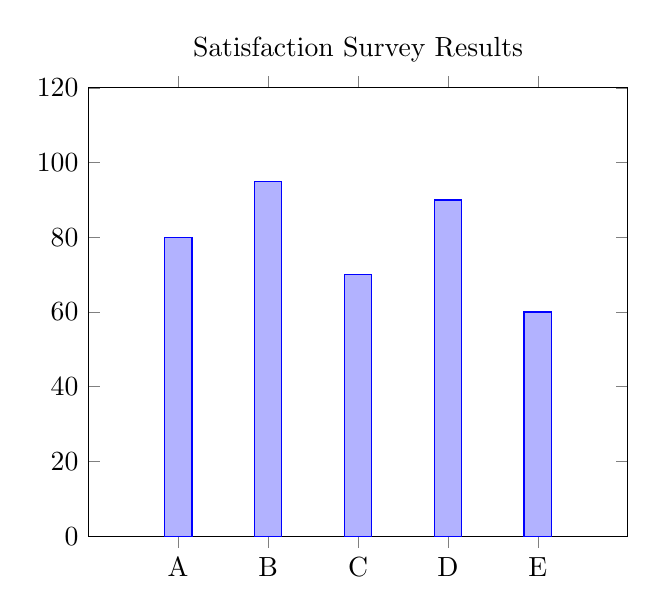
\begin{tikzpicture}
			\begin{axis}[
				ybar,
				enlarge x limits=0.25,
				symbolic x coords={A, B, C, D, E},
				xtick=data,
				nodes near coords align={vertical},
				ymin=0, ymax=120,
				title={Satisfaction Survey Results}
				]
				\addplot coordinates {
					(A, 80) % Service A had 80 satisfied customers
					(B, 95) % Service B had 95 satisfied customers
					(C, 70) % Service C had 70 satisfied customers
					(D, 90) % Service D had 90 satisfied customers
					(E, 60) % Service E had 60 satisfied customers
				};
			\end{axis}
		\end{tikzpicture}
	\end{figure}
	
\end{document}
